\chapter{Data visualization}\label{chap:data}

To visualize the data more easily, multiple tools were developed. An infographic displaying the relationships between tags and categories is created using FraMindmap (Sec. \ref{sec:map}) and pie charts (Sec. \ref{sec:camembert}) are plotted using a Python code to visualize the diversity of projects uploaded on the website. 

\section{Types \& Topics map}\label{sec:map}

The mind-map that links tags with their categories (Fig. \ref{fig:Topics_category} \& \ref{fig:Types_category}) is available in FraMindmap\footnote{FraMindmap Types \& Topics taxonomy: \href{https://framindmap.org/c/maps/1527084/edit}{https://framindmap.org/c/maps/1527084/edit}} (Fig. \ref{fig:framamindmap}). It can be easily downloaded as an SVG file or a PNG. A global taxonomy is also available\footnote{FraMindmap Global taxonomy: \href{https://framindmap.org/c/maps/1531458/edit}{https://framindmap.org/c/maps/1531458/edit}}.

/!\textbackslash \ To modify the mind-map, an account is needed. At the moment this document is written, no better alternative was found.

\begin{figure}[h!]
    \centering
    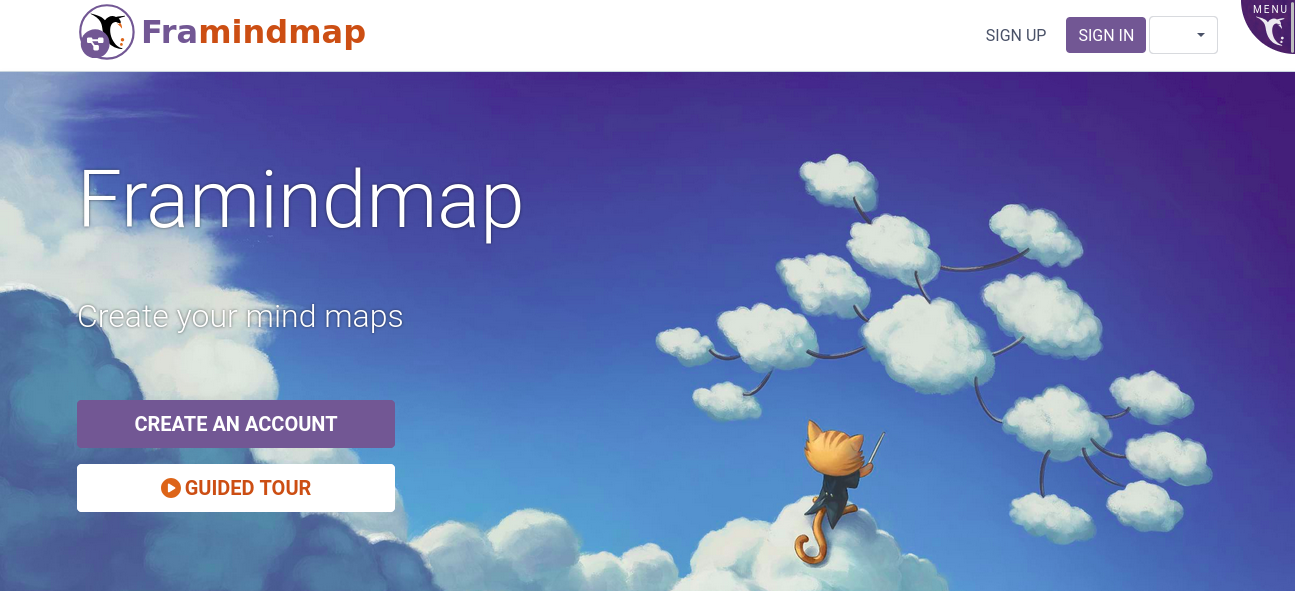
\includegraphics[width=\linewidth]{Image/Data visualization/framamindmap.png}
    \caption{Framindmap soft}
    \label{fig:framamindmap}
\end{figure}

\newpage
\section{Data visualization}\label{sec:camembert}

The code is available in GitHub: 
\begin{lstlisting}[language=Python]
    git clone https://github.com/Troy314/IPPOG_Website.git
\end{lstlisting}

\begin{itemize}
    \item \gray{data\_topics\_dictionary.py}, \gray{data\_types\_dictionary.py}, \gray{data\_representatives\_dictonary.py} are dictionaries that count respectively the topics and types of the projects as well as the IPPOG members related to each project. 
    \item \gray{data\_analysis\_local.py} \& \gray{data\_analysis\_online.py} files are the codes that create the graphs. They go through all items of the database of which [Status = "Online"] and display pie charts online projects.
    \item \gray{media/data} is the folder where graphs are saved as SVG files
\end{itemize}


Two versions of the code are available
\begin{itemize}
    \item \gray{data\_analysis\_local.py}: directly extract data through Google's API (need the optional dependencies)
    \item \gray{data\_analysis\_online.py}: extract data from a local CSV file 
\end{itemize}

\begin{multicols}{2}
    \raggedcolumns
    \subsubsection*{Online mode}
        
        /!\textbackslash \ Requires the use of Google API, see Sec. \ref{ssec:API}.\newline
        /!\textbackslash \ Requires optional dependencies, see Sec. \ref{dependencies}\newline
        /!\textbackslash \ The JSON file should be put in the same folder as the run file
            
        To run the program, simply run
        \begin{lstlisting}[language=Python]
        python3 data_analysis_online.py\end{lstlisting}
        \columnbreak
    \subsubsection*{Local mode}
        
        /!\textbackslash \ Requires to download the database available on Google sheet\footnote{Google Sheet: \href{https://docs.google.com/spreadsheets/d/1x_SdxdlHwG8chH77WqrTAAgijY2XBY3nPIi2p3TKqzs/edit?gid=1297224389\#gid=1297224389}{https://shorturl.at/sHBrz}} as a CSV file\newline
        /!\textbackslash \ The CSV file should be put in the same folder as the run file
        
        To run the program, simply run
        \begin{lstlisting}[language=Python]
        python3 data_analysis_local.py\end{lstlisting}
        
        The codes will then ask for the name of the CSV file containing the database.
\end{multicols}

The codes produce a \gray{media/data/} folder in which three SVG files are produced: 
\begin{itemize}
    \item Related members data (Fig. \ref{fig:members})
    \item Topics data (Fig. \ref{fig:topics})
    \item Types data (Fig. \ref{fig:types})
\end{itemize}